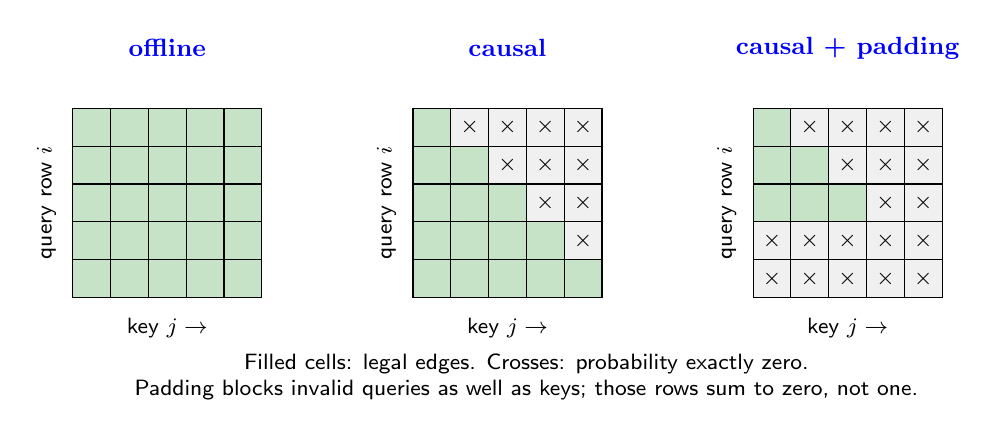
\begin{tikzpicture}[x=.48cm,y=.48cm,font=\footnotesize\sffamily]
\foreach \shift/\title in {0/offline,9/causal,18/{causal + padding}}{
\begin{scope}[xshift=\shift*.48cm]
\node[Blue,font=\small\bfseries] at (2.5,6.6) {\title};
\foreach \i in {0,...,4}\foreach \j in {0,...,4}{
\pgfmathtruncatemacro{\blocked}{0}
\ifnum\shift>0 \ifnum\j>\i \def\blocked{1}\fi\fi
\ifnum\shift=18 \ifnum\j>2 \def\blocked{1}\fi \ifnum\i>2 \def\blocked{1}\fi\fi
\ifnum\blocked=1 \draw[fill=gray!12] (\j,4-\i) rectangle ++(1,1);
\node at (\j+.5,4.5-\i) {$\times$};
\else \draw[fill=Green!22] (\j,4-\i) rectangle ++(1,1); \fi}
\node[below] at (2.5,-.3) {key $j\rightarrow$};
\node[rotate=90] at (-.7,2.5) {query row $i$};
\end{scope}}
\node[align=center] at (12,-2.1) {Filled cells: legal edges. Crosses: probability exactly zero.\\
Padding blocks invalid queries as well as keys; those rows sum to zero, not one.};
\end{tikzpicture}
